\section{行列式的定义及其性质}

行列式的性质可以帮助我们更加深入地理解行列式的本质, 同时也为行列式的计算提供了一些重要的技巧和方法.

\subsection{逆序数}

\begin{definition}[排列]
    $n $ 级排列由 $ 1,2, \cdots, n $ 组成的一个有序数组称为一个 $ n $ 级\textit{排列}, 通常记为 $ i_{1} i_{2} \cdots i_{n} $.
\end{definition}
\begin{definition}[逆序数]
    在一个排列中, 如果一对数的前后位置与大小顺序相反, 即前面的数大于后面的数, 则它们构成一个\textit{逆序}.
    一个排列中的逆序总数, 称为这个排列的逆序数, 通常记为 $ \tau\left(i_{1} i_{2} \cdots i_{n}\right) $.
\end{definition}
\begin{definition}[奇 (偶) 排列]
    逆序数为奇数 (偶数) 的排列, 称为奇 (偶) 排列.
\end{definition}
\begin{definition}[对换]
    把一个排列中某两个数的位置互换, 而其余的数不动, 就得到另一个排列, 这样的一个变换称为一次对换.
\end{definition}
\begin{theorem}
    任意一个排列经过一次对换后, 奇偶性改变.
\end{theorem}
\begin{theorem}
    $ n ~(n>1)$ 级排列共有 $ n! $ 种, 奇偶排列各占一半.
\end{theorem}

\begin{example}
    选择 $i$ 与 $k$, 使 $a_{1i}a_{32}a_{4k}a_{25}a_{53}$ 成为五阶行列式中一个带负号的项.
\end{example}
\begin{solution}
    将给定的项改写成行标自然顺序, 即 $$a_{1i}a_{25}a_{32}a_{4k}a_{53}$$
    列标构成的排列 $i52k4$ 中缺 $1$ 和 $4$, 令 $i=1,k=4,\tau(15243)=3+1=4$, 故该项带正号;
    令 $i=4,k=1,\tau(45213)=3+3+1=7$, 故该项带负号.
\end{solution}

\subsection{行列式的概念}

\begin{definition}[$n$ 阶行列式]
    $\mqty|a_{11} & a_{12} & \cdots & a_{1 n} \\ a_{21} & a_{22} & \cdots & a_{2 n} \\ \vdots & \vdots & & \vdots \\ a_{n 1} & a_{n 2} & \cdots & a_{n n}|$
    是所有取自不同行不同列的 $ n $ 个元素的乘积 $$ a_{1_{1}} a_{2 j_{2}} \cdots a_{n j_{n}} $$ 的代数和, 这里 $ j_{1} j_{2} \cdots j_{n} $ 是一个 $ n $ 级排列.
    当 $ j_{1} j_{2} \cdots j_{n} $ 是偶排列时, 该项前面带正号; 当 $ j_{1} j_{2} \cdots j_{n} $ 是奇排列时, 该项前面带负号, 即
    $$\mqty|a_{11}  & a_{12}  & \cdots & a_{1 n} \\
            a_{21}  & a_{22}  & \cdots & a_{2 n} \\
            \vdots  & \vdots  &        & \vdots  \\
            a_{n 1} & a_{n 2} & \cdots & a_{n n}|=\sum_{j_{1} j_{2} \cdots j_{n}}(-1)^{\tau\left(j_{j_{2}} \cdots j_{n}\right)} a_{1 j_{1}} a_{2 j_{2}} \cdots a_{n j_{n}}$$
    其中 $ \displaystyle\sum_{j_{1} j_{2} \cdots j_{n}} $ 表示对所有 $ n $ 级排列求和. $ n $ 阶行列式有时简记为 $ \left|a_{i j}\right|_{n} $, 而且有如下另外两种类似的定义:
    $$\left|a_{i j}\right|_{n}=\sum_{i_{1} i_{2} \cdots i_{n}}(-1)^{\tau\left(i_{1} i_{2} \cdots i_{n}\right)} a_{i_{1} 1} a_{i_{2} 2} \cdots a_{i_{n} n}$$
    和 $$\left|a_{i j}\right|_{n}=\sum_{\substack{i_{i} i_{2} \cdots i_{n} \\  j_{1} j_{2} \cdots j_{n}}}(-1)^{\tau\left(i_{1} i_{2} \cdots i_{n}\right)+\tau\left(j_{j_{2}} \cdots \cdot j_{n}\right)} a_{i_{1} j_{1}} a_{i_{2} j_{2}} \cdots a_{i_{n_{n}} j_{n}} .$$
\end{definition}

由 $ n $ 级排列的性质可知, $n $ 阶行列式共有 $ n! $ 项, 其中冠以正号的项和冠以负号的项 (不算元素本身所带的负号) 各占一半.

\begin{example}
    求 $\displaystyle f(x)=\begin{vmatrix}
            2x & x & 1 & 2  \\
            1  & x & 1 & -1 \\
            3  & 2 & x & 1  \\
            1  & 1 & 1 & x
        \end{vmatrix}$ 中 $x^4$ 与 $x^3$ 的系数.
\end{example}
\begin{solution}
    只有行列式的对角线上的元素相乘才出现 $x^4$, 并且带正号, 于是 $x^4$ 的系数为 $2$;
    同理, 含 $x^3$ 的项只有一项, 即 $$x\cdot 1\cdot x\cdot x=x^3$$
    而且其列标所构成的排列为 $2134$, 于是 $\tau(2134)=1$, 即 $x^3$ 的系数为 $-1.$
\end{solution}

\begin{example}
    \label{n jie hang lie shi wei fen fa}
    证明 $n$ 阶行列式微分法:
    $$\frac{\dd  }{\dd  x} \begin{vmatrix}
            f_{11} & f_{12} & \cdots & f_{1n} \\
            \vdots & \vdots &        & \vdots \\
            f_{i1} & f_{i2} & \cdots & f_{in} \\
            \vdots & \vdots &        & \vdots \\
            f_{n1} & f_{n2} & \cdots & f_{nn}
        \end{vmatrix}=\sum_{i=1}^{n}
        \begin{vmatrix}
            f_{11}                       & f_{12}                      & \cdots & f_{1n}                       \\
            \vdots                       & \vdots                      &        & \vdots                       \\
            \dfrac{\dd  }{\dd x } f_{i1} & \dfrac{\dd  }{\dd x }f_{i2} & \cdots & \dfrac{\dd  }{\dd x } f_{in} \\
            \vdots                       & \vdots                      &        & \vdots                       \\
            f_{n1}                       & f_{n2}                      & \cdots & f_{nn}
        \end{vmatrix}.$$
\end{example}
\begin{proof}[{\songti \textbf{证}}]
    从行列式的定义出发予以证明, 
    \begin{flalign*}
         & \frac{\dd  }{\dd  x}
        \begin{vmatrix}
            f_{11} & f_{12} & \cdots & f_{1n} \\
            \vdots & \vdots &        & \vdots \\
            f_{i1} & f_{i2} & \cdots & f_{in} \\
            \vdots & \vdots &        & \vdots \\
            f_{n1} & f_{n2} & \cdots & f_{nn}
        \end{vmatrix}
        =\dfrac{\dd }{\dd x}\sum_{j_1~j_2~\cdots ~j_n}(-1)^{\tau (j_1~j_2~\cdots ~j_n)}\prod_{i=1}^{n}f_{i~j_i}                                                                                                                                                  \\
         & =\sum_{j_1~j_2~\cdots ~j_n}(-1)^{\tau (j_1~j_2~\cdots ~j_n)}\dfrac{\dd }{\dd x}\prod_{i=1}^{n}f_{i~j_i}=\sum_{j_1~j_2~\cdots ~j_n}(-1)^{\tau (j_1~j_2~\cdots ~j_n)}\sum_{i=1}^{n}f_{1~j_1}f_{2~j_2}\cdots\dfrac{\dd }{\dd x}f_{i~j_i}\cdots f_{n~j_n} \\
         & =\sum_{i=1}^{n}\sum_{j_1~j_2~\cdots ~j_n}(-1)^{\tau (j_1~j_2~\cdots ~j_n)}f_{1~j_1}f_{2~j_2}\cdots\dfrac{\dd }{\dd x}f_{i~j_i}\cdots f_{n~j_n}=\sum_{i=1}^{n}
        \begin{vmatrix}
            f_{11}                       & f_{12}                      & \cdots & f_{1n}                       \\
            \vdots                       & \vdots                      &        & \vdots                       \\
            \dfrac{\dd  }{\dd x } f_{i1} & \dfrac{\dd  }{\dd x }f_{i2} & \cdots & \dfrac{\dd  }{\dd x } f_{in} \\
            \vdots                       & \vdots                      &        & \vdots                       \\
            f_{n1}                       & f_{n2}                      & \cdots & f_{nn}
        \end{vmatrix}.
    \end{flalign*}
\end{proof}

\subsection{行列式的基本性质}

\begin{theorem}[行列式的转置]
    行列式 $ D $ 与它的转置行列式 $ D^{\top} $ (将 $ D $ 行的项转为列的项, 如第 1 行转为第 1 列, $ \cdots $, 第 $ n $ 行转为第 $ n $ 列) 相等.
\end{theorem}
\begin{theorem}[变号定理]
    互换行列式的两行 (列), 行列式变号 (例如, 交换第 1 行和第 2 行, 记为 $ r_{1} \leftrightarrow r_{2} $; 交换第 1 列和第 2 列, 
    记为 $ c_{1} \leftrightarrow c_{2} $).
\end{theorem}
\begin{theorem}[行列式的数乘]
    行列式的某一行(列) 中所有的元素都乘以同一数 $ k $, 等于用数 $ k $ 乘此行列式.
\end{theorem}
\begin{inference}
    行列式中某一行 (列) 的所有元素的公因子可以提到整个行列式的外面.
\end{inference}
\begin{theorem}
    行列式中如果有两行 (列) 元素成比例, 则此行列式等于零.
\end{theorem}
\begin{theorem}[行列式拆分]
    若行列式的某一列 (行) 的所有元素都是两数之和, 例如第 $ i $ 列的元素都是两数之和, 即
    $$\begin{vmatrix}
            a_{11} & a_{12} & \cdots & a_{1i}+a_{1i}' & \cdots & a_{1n} \\
            a_{21} & a_{22} & \cdots & a_{2i}+a_{2i}' & \cdots & a_{2n} \\
            \vdots & \vdots &        & \vdots         &        & \vdots \\
            a_{n1} & a_{22} & \cdots & a_{ni}+a_{ni}' & \cdots & a_{2n} \\
        \end{vmatrix}$$
    则 $D$ 等于下列两个行列式之和
    $$D=\begin{vmatrix}
            a_{11} & a_{12} & \cdots & a_{1i} & \cdots & a_{1n} \\
            a_{21} & a_{22} & \cdots & a_{2i} & \cdots & a_{2n} \\
            \vdots & \vdots &        & \vdots &        & \vdots \\
            a_{n1} & a_{22} & \cdots & a_{2i} & \cdots & a_{nn} \\
        \end{vmatrix}
        =\begin{vmatrix}
            a_{11} & a_{12} & \cdots & a_{1i}' & \cdots & a_{1n} \\
            a_{21} & a_{22} & \cdots & a_{2i}' & \cdots & a_{2n} \\
            \vdots & \vdots &        & \vdots  &        & \vdots \\
            a_{n1} & a_{22} & \cdots & a_{ni}' & \cdots & a_{nn} \\
        \end{vmatrix}$$
\end{theorem}
\begin{theorem}[行列式变换]
    把行列式的某一行 (列) 的各元素乘以同一数然后加到另一行 (列) 对应的元素上, 行列式不变.
\end{theorem}

\begin{example}
    设矩阵 $\vb*{A}=\begin{pmatrix} a_{11} & a_{12} & 1 \\ a_{21} & a_{22} & 1 \\ a_{31} & a_{32} & 1 \\\end{pmatrix},~y=f(x)$ 是连续函数, 点 $A_{i}(a_{i1},a_{i2})~(i=1,2,3)$ 为曲线 $y=f(x)$ 上三个不同点, 记三角形 $\bigtriangleup A_1A_2A_3$ 的面积为 $S_{\bigtriangleup A_1A_2A_3}$, 则下列说法正确的是 (\quad).
    \begin{tasks}(2)
        \task $\rank\vb*{A}=1\text{ 或 }2,~\det\vb*{A}=S_{\bigtriangleup A_1A_2A_3}$
        \task $\rank\vb*{A}=1\text{ 或 }2,~\det\vb*{A}=2S_{\bigtriangleup A_1A_2A_3}$
        \task $\rank\vb*{A}=2\text{ 或 }3,~\det\vb*{A}=S_{\bigtriangleup A_1A_2A_3}$
        \task $\rank\vb*{A}=2\text{ 或 }3,~\det\vb*{A}=2S_{\bigtriangleup A_1A_2A_3}$
    \end{tasks}
\end{example}

\begin{solution}
    如图 \ref{sjiehanglsyouxtji} 所示, 含 “1” 列的三阶行列式等于平行六面体 $P-OA_1A_2A_3$ 的有向体积, 当 $\overrightarrow{OA_1} ,\overrightarrow{OA_2} ,\overrightarrow{OA_3} $ 共面不共线时, 该平行六面体的体积为 $0$, 且 $\rank\vb*{A}=2$, 当 $\overrightarrow{OA_1} ,\overrightarrow{OA_2} ,\overrightarrow{OA_3} $ 不共面时, $\rank\vb*{A}=3$.
    \begin{figure}[H]
        \centering
        \tikzset{every picture/.style={line width=0.75pt}} %set default line width to 0.75pt        

        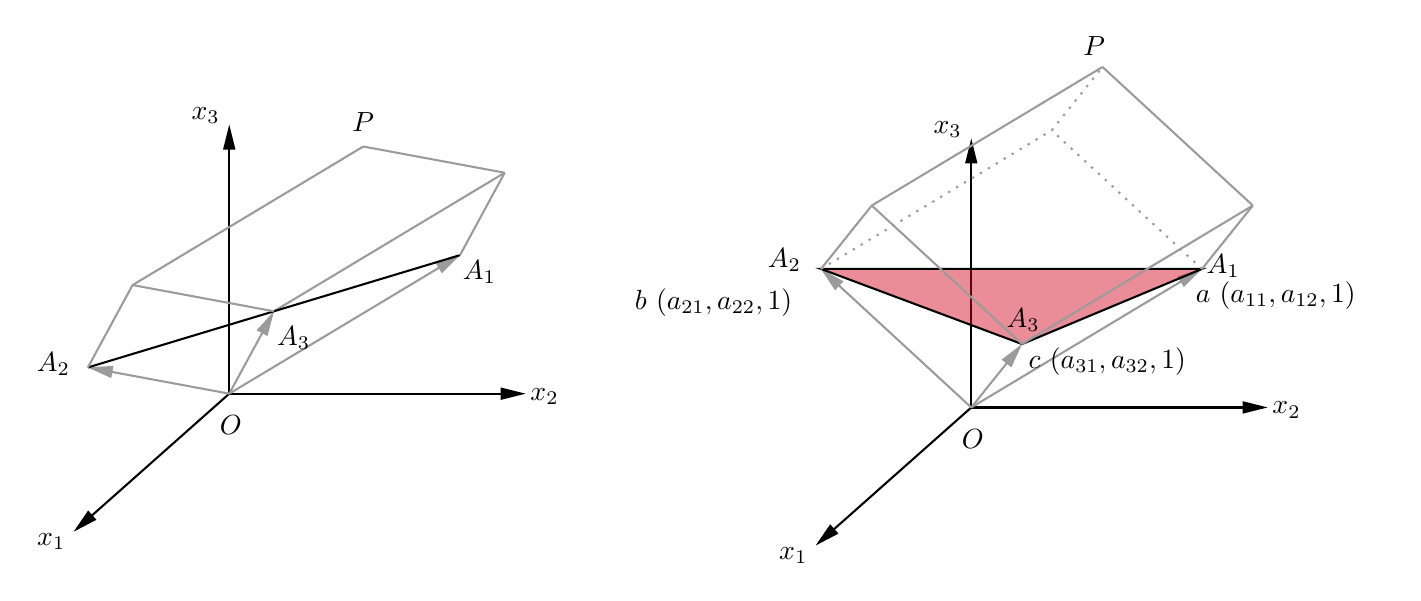
\begin{tikzpicture}[x=0.75pt,y=0.75pt,yscale=-1,xscale=1]
        %uncomment if require: \path (0,300); %set diagram left start at 0, and has height of 300

        %Straight Lines [id:da20382206865087626] 
        \draw    (491.34,197.81) -- (632.12,197.81) ;
        \draw [shift={(634.12,197.81)}, rotate = 180] [fill={rgb, 255:red, 0; green, 0; blue, 0 }  ][line width=0.08]  [draw opacity=0] (12,-3) -- (0,0) -- (12,3) -- cycle    ;
        %Straight Lines [id:da18857754521279135] 
        \draw    (491.34,197.81) -- (417.87,262.97) ;
        \draw [shift={(416.38,264.3)}, rotate = 318.43] [fill={rgb, 255:red, 0; green, 0; blue, 0 }  ][line width=0.08]  [draw opacity=0] (12,-3) -- (0,0) -- (12,3) -- cycle    ;
        %Straight Lines [id:da7776725180589441] 
        \draw    (491.34,197.81) -- (491.34,70.2) ;
        \draw [shift={(491.34,68.2)}, rotate = 90] [fill={rgb, 255:red, 0; green, 0; blue, 0 }  ][line width=0.08]  [draw opacity=0] (12,-3) -- (0,0) -- (12,3) -- cycle    ;
        %Straight Lines [id:da6633859303056509] 
        \draw [color={rgb, 255:red, 155; green, 155; blue, 155 }  ,draw opacity=1 ]   (491.34,197.81) -- (600.79,132.09) ;
        \draw [shift={(602.5,131.06)}, rotate = 149.01] [fill={rgb, 255:red, 155; green, 155; blue, 155 }  ,fill opacity=1 ][line width=0.08]  [draw opacity=0] (12,-3) -- (0,0) -- (12,3) -- cycle    ;
        %Straight Lines [id:da00562488690732188] 
        \draw [color={rgb, 255:red, 155; green, 155; blue, 155 }  ,draw opacity=1 ]   (491.34,197.81) -- (514.56,168.83) ;
        \draw [shift={(515.81,167.27)}, rotate = 128.71] [fill={rgb, 255:red, 155; green, 155; blue, 155 }  ,fill opacity=1 ][line width=0.08]  [draw opacity=0] (12,-3) -- (0,0) -- (12,3) -- cycle    ;
        %Straight Lines [id:da46359590583857657] 
        \draw [color={rgb, 255:red, 155; green, 155; blue, 155 }  ,draw opacity=1 ]   (491.34,197.81) -- (420.4,132.42) ;
        \draw [shift={(418.93,131.06)}, rotate = 42.67] [fill={rgb, 255:red, 155; green, 155; blue, 155 }  ,fill opacity=1 ][line width=0.08]  [draw opacity=0] (12,-3) -- (0,0) -- (12,3) -- cycle    ;
        %Shape: Polygon [id:ds25999654756750057] 
        \draw  [color={rgb, 255:red, 0; green, 0; blue, 0 }  ,draw opacity=1 ][fill={rgb, 255:red, 208; green, 2; blue, 27 }  ,fill opacity=0.45 ] (418.93,131.06) -- (602.5,131.06) -- (515.81,167.27) -- cycle ;
        %Straight Lines [id:da6498067396133682] 
        \draw [color={rgb, 255:red, 155; green, 155; blue, 155 }  ,draw opacity=1 ]   (602.5,131.06) -- (626.98,100.52) ;
        %Straight Lines [id:da6398150627428405] 
        \draw [color={rgb, 255:red, 155; green, 155; blue, 155 }  ,draw opacity=1 ]   (515.81,167.27) -- (443.4,100.52) ;
        %Straight Lines [id:da4103254568966608] 
        \draw [color={rgb, 255:red, 155; green, 155; blue, 155 }  ,draw opacity=1 ]   (418.93,131.06) -- (443.4,100.52) ;
        %Straight Lines [id:da8745871832428125] 
        \draw [color={rgb, 255:red, 155; green, 155; blue, 155 }  ,draw opacity=1 ]   (515.81,167.27) -- (626.98,100.52) ;
        %Straight Lines [id:da9014665955789909] 
        \draw [color={rgb, 255:red, 155; green, 155; blue, 155 }  ,draw opacity=1 ]   (626.98,100.52) -- (554.57,33.76) ;
        %Straight Lines [id:da31721325149361723] 
        \draw [color={rgb, 255:red, 155; green, 155; blue, 155 }  ,draw opacity=1 ]   (443.4,100.52) -- (554.57,33.76) ;
        %Straight Lines [id:da5853440026382923] 
        \draw [color={rgb, 255:red, 155; green, 155; blue, 155 }  ,draw opacity=1 ] [dash pattern={on 0.84pt off 2.51pt}]  (530.09,64.3) -- (554.57,33.76) ;
        %Straight Lines [id:da018444457149563] 
        \draw [color={rgb, 255:red, 155; green, 155; blue, 155 }  ,draw opacity=1 ] [dash pattern={on 0.84pt off 2.51pt}]  (418.93,131.06) -- (530.09,64.3) ;
        %Straight Lines [id:da37422004513113794] 
        \draw [color={rgb, 255:red, 155; green, 155; blue, 155 }  ,draw opacity=1 ] [dash pattern={on 0.84pt off 2.51pt}]  (602.5,131.06) -- (530.09,64.3) ;
        %Straight Lines [id:da6574486979884699] 
        \draw    (133.84,191.17) -- (274.62,191.17) ;
        \draw [shift={(276.62,191.17)}, rotate = 180] [fill={rgb, 255:red, 0; green, 0; blue, 0 }  ][line width=0.08]  [draw opacity=0] (12,-3) -- (0,0) -- (12,3) -- cycle    ;
        %Straight Lines [id:da1818030714615222] 
        \draw    (133.84,191.17) -- (60.38,256.33) ;
        \draw [shift={(58.88,257.65)}, rotate = 318.43] [fill={rgb, 255:red, 0; green, 0; blue, 0 }  ][line width=0.08]  [draw opacity=0] (12,-3) -- (0,0) -- (12,3) -- cycle    ;
        %Straight Lines [id:da8683567459389139] 
        \draw    (133.84,191.17) -- (133.84,63.56) ;
        \draw [shift={(133.84,61.56)}, rotate = 90] [fill={rgb, 255:red, 0; green, 0; blue, 0 }  ][line width=0.08]  [draw opacity=0] (12,-3) -- (0,0) -- (12,3) -- cycle    ;
        %Straight Lines [id:da06489442305353244] 
        \draw [color={rgb, 255:red, 155; green, 155; blue, 155 }  ,draw opacity=1 ]   (133.84,191.17) -- (243.29,125.45) ;
        \draw [shift={(245.01,124.42)}, rotate = 149.01] [fill={rgb, 255:red, 155; green, 155; blue, 155 }  ,fill opacity=1 ][line width=0.08]  [draw opacity=0] (12,-3) -- (0,0) -- (12,3) -- cycle    ;
        %Straight Lines [id:da8445420371786283] 
        \draw [color={rgb, 255:red, 155; green, 155; blue, 155 }  ,draw opacity=1 ]   (133.84,191.17) -- (154.42,153.23) ;
        \draw [shift={(155.37,151.47)}, rotate = 118.47] [fill={rgb, 255:red, 155; green, 155; blue, 155 }  ,fill opacity=1 ][line width=0.08]  [draw opacity=0] (12,-3) -- (0,0) -- (12,3) -- cycle    ;
        %Straight Lines [id:da172209488567292] 
        \draw [color={rgb, 255:red, 155; green, 155; blue, 155 }  ,draw opacity=1 ]   (133.84,191.17) -- (67.7,178.9) ;
        \draw [shift={(65.73,178.53)}, rotate = 10.51] [fill={rgb, 255:red, 155; green, 155; blue, 155 }  ,fill opacity=1 ][line width=0.08]  [draw opacity=0] (12,-3) -- (0,0) -- (12,3) -- cycle    ;
        %Straight Lines [id:da5713393377025349] 
        \draw [color={rgb, 255:red, 155; green, 155; blue, 155 }  ,draw opacity=1 ]   (155.37,151.47) -- (266.53,84.72) ;
        %Straight Lines [id:da3376780505283008] 
        \draw [color={rgb, 255:red, 155; green, 155; blue, 155 }  ,draw opacity=1 ]   (87.26,138.84) -- (198.43,72.08) ;
        %Straight Lines [id:da7556237923546365] 
        \draw    (65.73,178.53) -- (245.01,124.42) ;
        %Straight Lines [id:da07651078675235445] 
        \draw [color={rgb, 255:red, 155; green, 155; blue, 155 }  ,draw opacity=1 ]   (245.01,124.42) -- (266.53,84.72) ;
        %Straight Lines [id:da5032917543193056] 
        \draw [color={rgb, 255:red, 155; green, 155; blue, 155 }  ,draw opacity=1 ]   (65.73,178.53) -- (87.26,138.84) ;
        %Straight Lines [id:da30030976087464056] 
        \draw [color={rgb, 255:red, 155; green, 155; blue, 155 }  ,draw opacity=1 ]   (155.37,151.47) -- (87.26,138.84) ;
        %Straight Lines [id:da8146925186002858] 
        \draw [color={rgb, 255:red, 155; green, 155; blue, 155 }  ,draw opacity=1 ]   (266.53,84.72) -- (198.43,72.08) ;

        % Text Node
        \draw (619.81,129.84) node   [align=left] {\begin{minipage}[lt]{22.54pt}\setlength\topsep{0pt}
        $\displaystyle A_{1}$
        \end{minipage}};
        % Text Node
        \draw (408.35,126.86) node   [align=left] {\begin{minipage}[lt]{22.54pt}\setlength\topsep{0pt}
        $\displaystyle A_{2}$
        \end{minipage}};
        % Text Node
        \draw (523.38,155.82) node   [align=left] {\begin{minipage}[lt]{22.54pt}\setlength\topsep{0pt}
        $\displaystyle A_{3}$
        \end{minipage}};
        % Text Node
        \draw (501.83,213.03) node   [align=left] {\begin{minipage}[lt]{22.54pt}\setlength\topsep{0pt}
        $\displaystyle O$
        \end{minipage}};
        % Text Node
        \draw (413.83,268.98) node   [align=left] {\begin{minipage}[lt]{22.54pt}\setlength\topsep{0pt}
        $\displaystyle x_{1}$
        \end{minipage}};
        % Text Node
        \draw (651.49,199.05) node   [align=left] {\begin{minipage}[lt]{22.54pt}\setlength\topsep{0pt}
        $\displaystyle x_{2}$
        \end{minipage}};
        % Text Node
        \draw (488.25,63.88) node   [align=left] {\begin{minipage}[lt]{22.54pt}\setlength\topsep{0pt}
        $\displaystyle x_{3}$
        \end{minipage}};
        % Text Node
        \draw (644.71,143.94) node   [align=left] {\begin{minipage}[lt]{67.81pt}\setlength\topsep{0pt}
        $\displaystyle {\textstyle \boldsymbol{a} \ ( a_{11} ,a_{12} ,1)}$
        \end{minipage}};
        % Text Node
        \draw (375.32,147.09) node   [align=left] {\begin{minipage}[lt]{69.02pt}\setlength\topsep{0pt}
        $\displaystyle {\textstyle \boldsymbol{b} \ ( a_{21} ,a_{22} ,1)}$
        \end{minipage}};
        % Text Node
        \draw (563.73,175.82) node   [align=left] {\begin{minipage}[lt]{67.09pt}\setlength\topsep{0pt}
        $\displaystyle {\textstyle \boldsymbol{c} \ ( a_{31} ,a_{32} ,1)}$
        \end{minipage}};
        % Text Node
        \draw (553.07,23.83) node   [align=left] {\begin{minipage}[lt]{11.56pt}\setlength\topsep{0pt}
        $\displaystyle P$
        \end{minipage}};
        % Text Node
        \draw (261.38,132.64) node   [align=left] {\begin{minipage}[lt]{22.54pt}\setlength\topsep{0pt}
        $\displaystyle A_{1}$
        \end{minipage}};
        % Text Node
        \draw (56.19,176.88) node   [align=left] {\begin{minipage}[lt]{22.54pt}\setlength\topsep{0pt}
        $\displaystyle A_{2}$
        \end{minipage}};
        % Text Node
        \draw (171.88,164.51) node   [align=left] {\begin{minipage}[lt]{22.54pt}\setlength\topsep{0pt}
        $\displaystyle A_{3}$
        \end{minipage}};
        % Text Node
        \draw (144.33,206.39) node   [align=left] {\begin{minipage}[lt]{22.54pt}\setlength\topsep{0pt}
        $\displaystyle O$
        \end{minipage}};
        % Text Node
        \draw (56.33,262.33) node   [align=left] {\begin{minipage}[lt]{22.54pt}\setlength\topsep{0pt}
        $\displaystyle x_{1}$
        \end{minipage}};
        % Text Node
        \draw (294,192.41) node   [align=left] {\begin{minipage}[lt]{22.54pt}\setlength\topsep{0pt}
        $\displaystyle x_{2}$
        \end{minipage}};
        % Text Node
        \draw (130.76,57.24) node   [align=left] {\begin{minipage}[lt]{22.54pt}\setlength\topsep{0pt}
        $\displaystyle x_{3}$
        \end{minipage}};
        % Text Node
        \draw (200.91,60.51) node   [align=left] {\begin{minipage}[lt]{11.56pt}\setlength\topsep{0pt}
        $\displaystyle P$
        \end{minipage}};


        \end{tikzpicture}
        \caption{}
        \label{sjiehanglsyouxtji}
    \end{figure}
    又因为 $$\begin{vmatrix} a_{11} & a_{12} & 1 \\ a_{21} & a_{22} & 1 \\ a_{31} & a_{32} & 1 \\\end{vmatrix}=\begin{vmatrix} a_{11} & a_{12} & 1 \\ a_{21}-a_{11} & a_{22}-a_{12} & 0 \\ a_{31}-a_{11} & a_{32}-a_{12} & 0 \\\end{vmatrix}=\begin{vmatrix} a_{21}-a_{11} & a_{22}-a_{12} \\ a_{31}-a_{11} & a_{32}-a_{12} \\\end{vmatrix}$$
    二阶行列式 $\begin{vmatrix} a_{21}-a_{11} & a_{22}-a_{12} \\ a_{31}-a_{11} & a_{32}-a_{12} \\\end{vmatrix}$ 的向量张成的面实际上是在二维平面 $x_3=1$ 上, 
    即由行向量 $\overrightarrow{A_1A_2} =( a_{21}-a_{11} , a_{22}-a_{12} )$ 和 $\overrightarrow{A_1A_3} =(a_{31}-a_{11} , a_{32}-a_{12} )$ 所张成的平行四边形的有向面积, 而该平行四边形的有向面积等于 $2S_{\bigtriangleup A_1A_2A_3}$, 因此选 D.
\end{solution}

\subsection{几种特殊的行列式}

常见的行列式展开.
\setcounter{magicrownumbers}{0}
\begin{table}[H]
    \centering
    \caption{常见的行列式展开}
    \begin{tabular}{l}
        上三角形、下三角形、对角行列式                                                                                                                             \\
        (\rownumber) $\mqty|a_{11}         &        &        & *       \\
                                                   & a_{22} &        &         \\
                                                   &        & \ddots &         \\
                                    \boldsymbol{O} &        &        & a_{n n}|
            =\mqty|a_{11} &        &        & \boldsymbol{O} \\
                              & a_{22} &        &                \\
                              &        & \ddots &                \\
                       *      &        &        & a_{n n}|
        =\mqty|a_{11}         &        &        & \boldsymbol{O} \\
                                      & a_{22} &        &                \\
                                      &        & \ddots &                \\
                       \boldsymbol{O} &        &        & a_{n n}|=a_{11} a_{22} \cdots a_{n n}$                                                                                                   \\
        \midrule
        副对角线方向的行列式                                                                                                                                       \\
        (\rownumber) $\begin{vmatrix}
                              *      &                                        &           & a_{1n}         \\
                                     &                                        & a_{2,n-1} &                \\
                                     & \begin{sideways}$\ddots$\end{sideways} &           &                \\
                              a_{n1} &                                        &           & \boldsymbol{O}
                          \end{vmatrix}
            =\begin{vmatrix}
                 \boldsymbol{O} &                                        &           & a_{1n} \\
                                &                                        & a_{2,n-1} &        \\
                                & \begin{sideways}$\ddots$\end{sideways} &           &        \\
                 a_{n1}         &                                        &           & *
             \end{vmatrix}
        =\begin{vmatrix}
                 \boldsymbol{O} &                                        &           & a_{1n}         \\
                                &                                        & a_{2,n-1} &                \\
                                & \begin{sideways}$\ddots$\end{sideways} &           &                \\
                 a_{n1}         &                                        &           & \boldsymbol{O}
             \end{vmatrix}$                                                                      \\
        $=(-1)^{\frac{n(n-1)}{2}}\displaystyle\prod_{i=1}^{n}a_{i,n-i+1}$
    \end{tabular}
\end{table}